\section{Solenoid and Torus Magnets}


\subsection{Geometry}
The solenoid geometry is produced with the GEMC perl api. The solenoid is a single polycone volume, shown in \F{solenoid}
in a section view with the target and an 11 GeV electron beam.

\begin{figure}
	\centering
	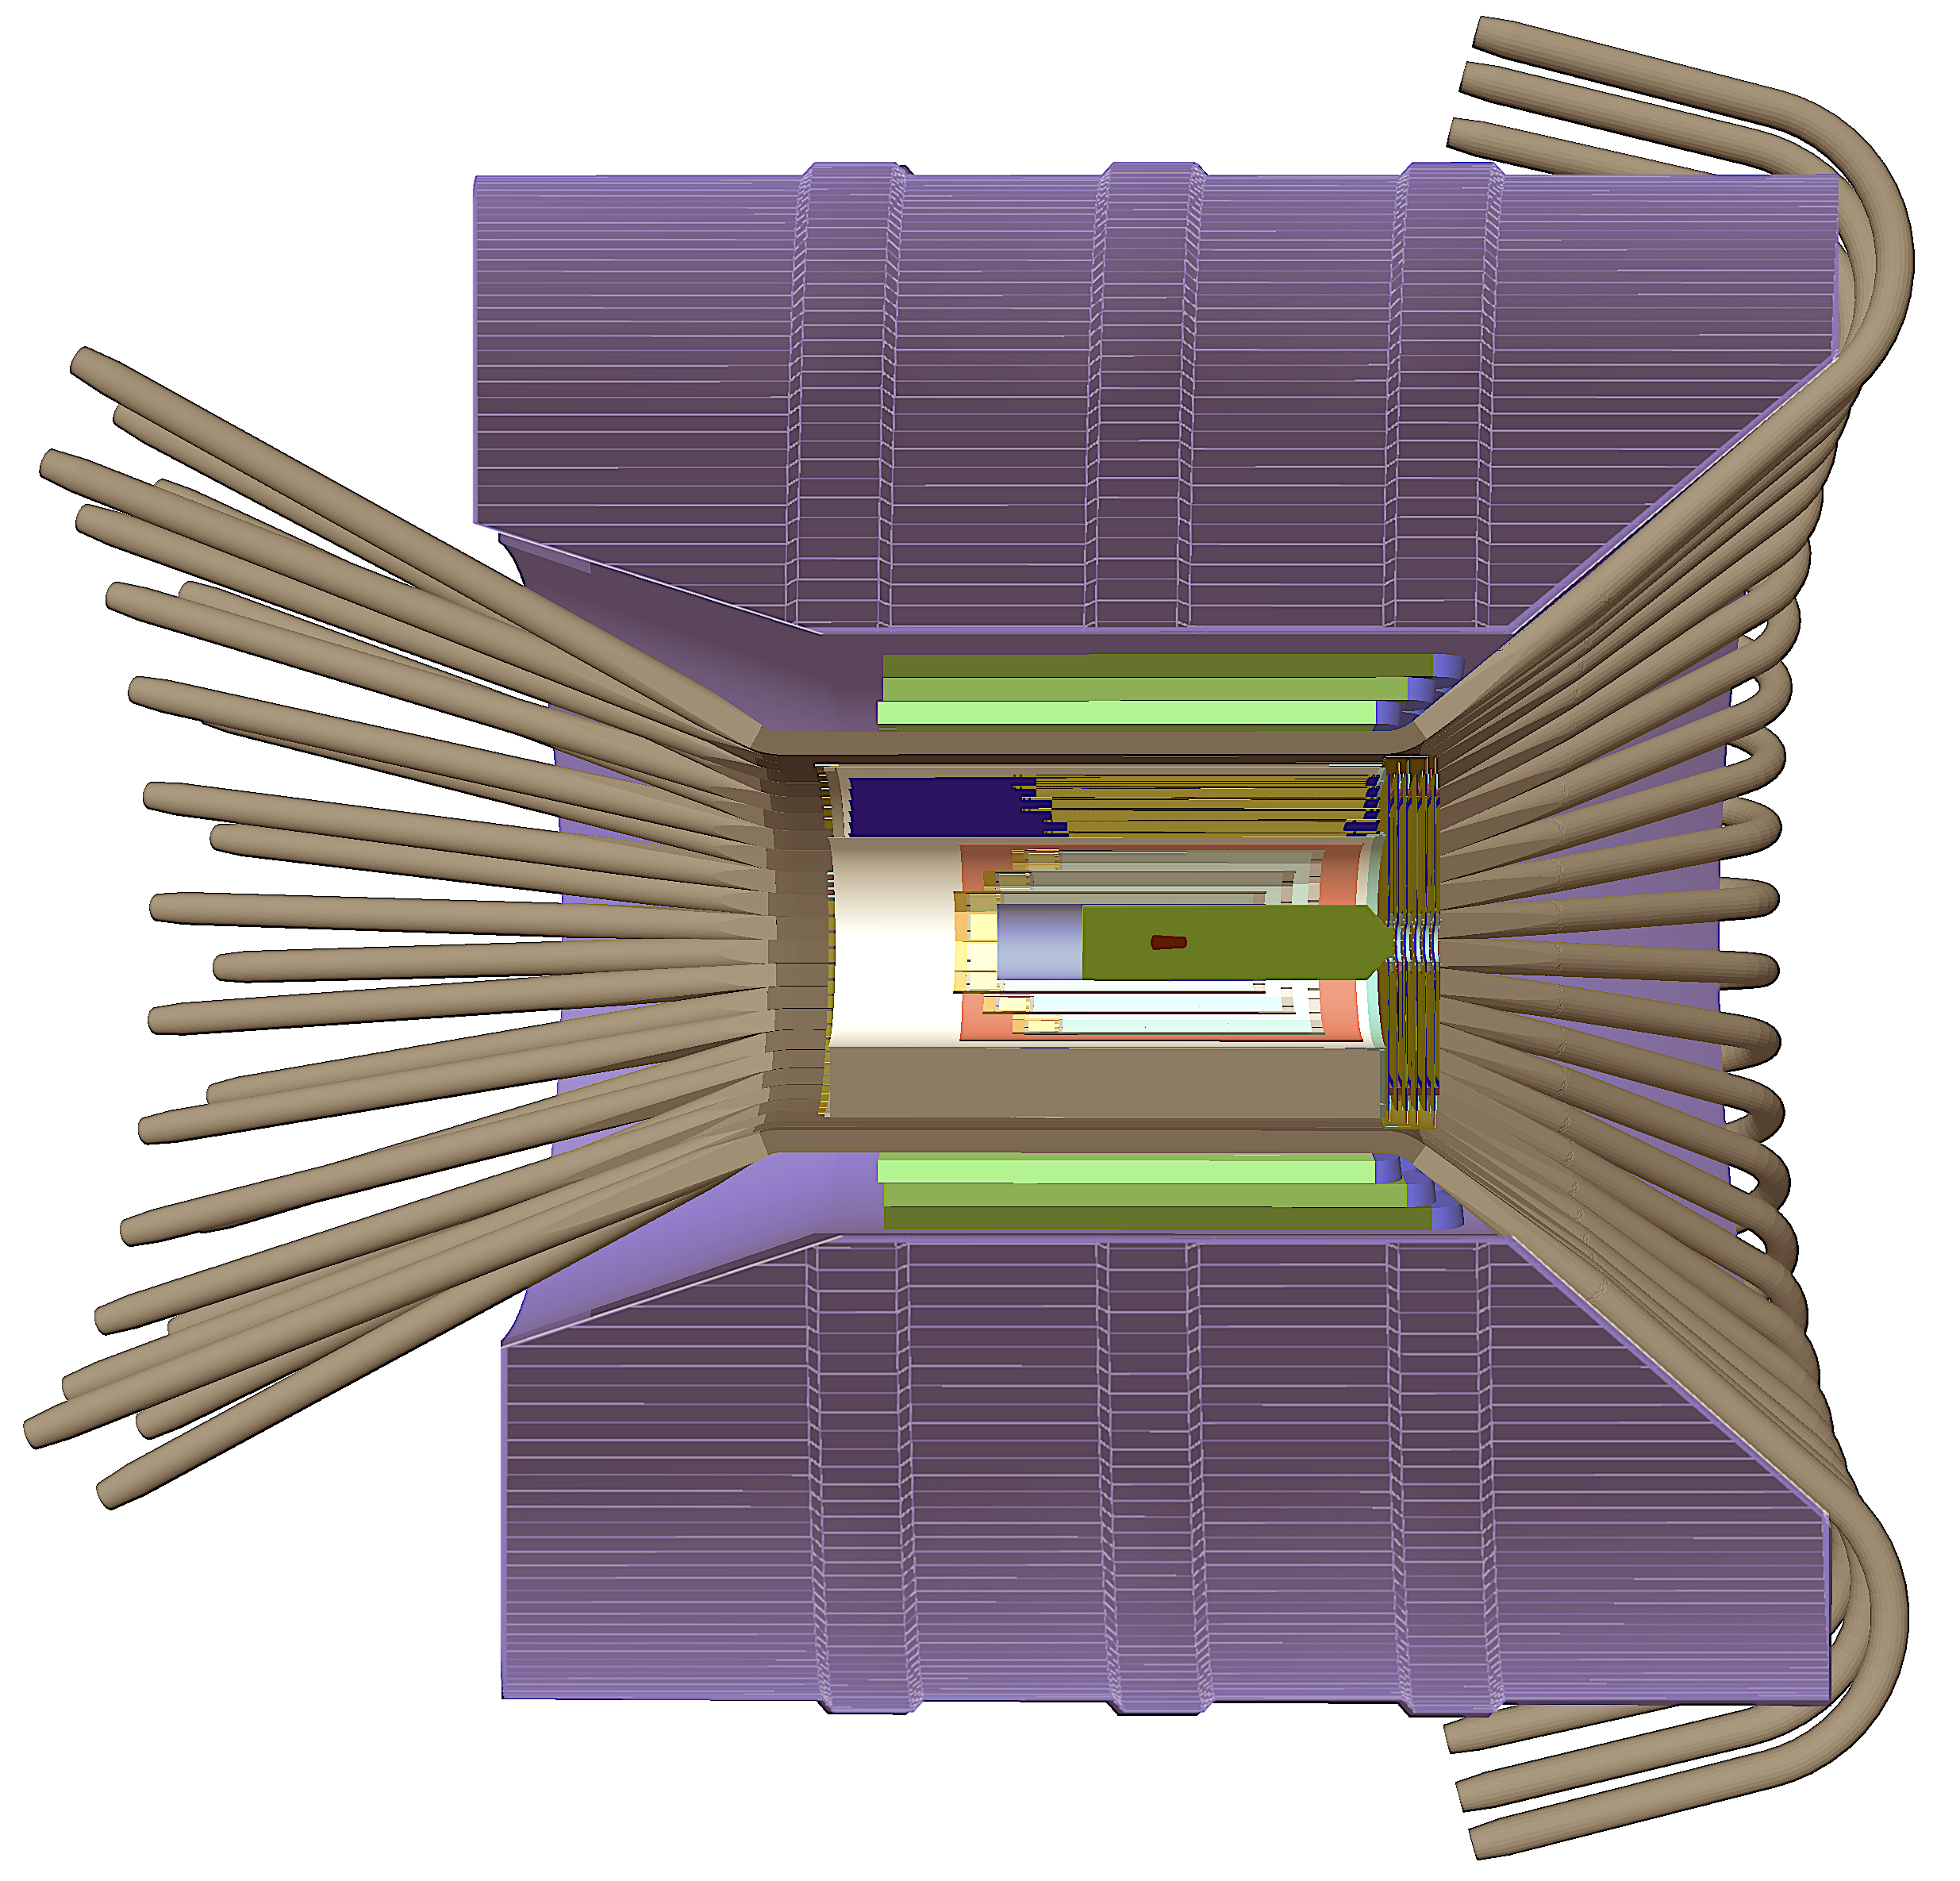
\includegraphics[width=0.98\columnwidth,keepaspectratio]{img/solenoid.png}
   \caption{An 11 GeV electron beam is impinging on a 5 cm liquid hydrogen target. At the full $10^{35} cm-2s-1$ luminosity, this correspond to
            124,000 electrons in a 250 ns window. Normally this would produce a storm of moeller electrons that would saturate any detector in the forward or central
				region. However the solenoid focus all of them along the beam line, providing the most effective shield to CLAS12.
            }
	\label{fig:solenoid}
\end{figure}

The torus geometry is imported from the engineering CAD model through 54 tessellated volumes. Among the volumes:

\begin{itemize}
	\item the bore heat shield and hub components
	\item the back and front plants
	\item the stainless steel coil frames
	\item the copper coils
	\item internal shielding around the hub
\end{itemize}

The torus hub is protected from the beampipe background with additional tungsten shielding.
The torus geometry is shown in \F{torus}.

\begin{figure}
	\centering
	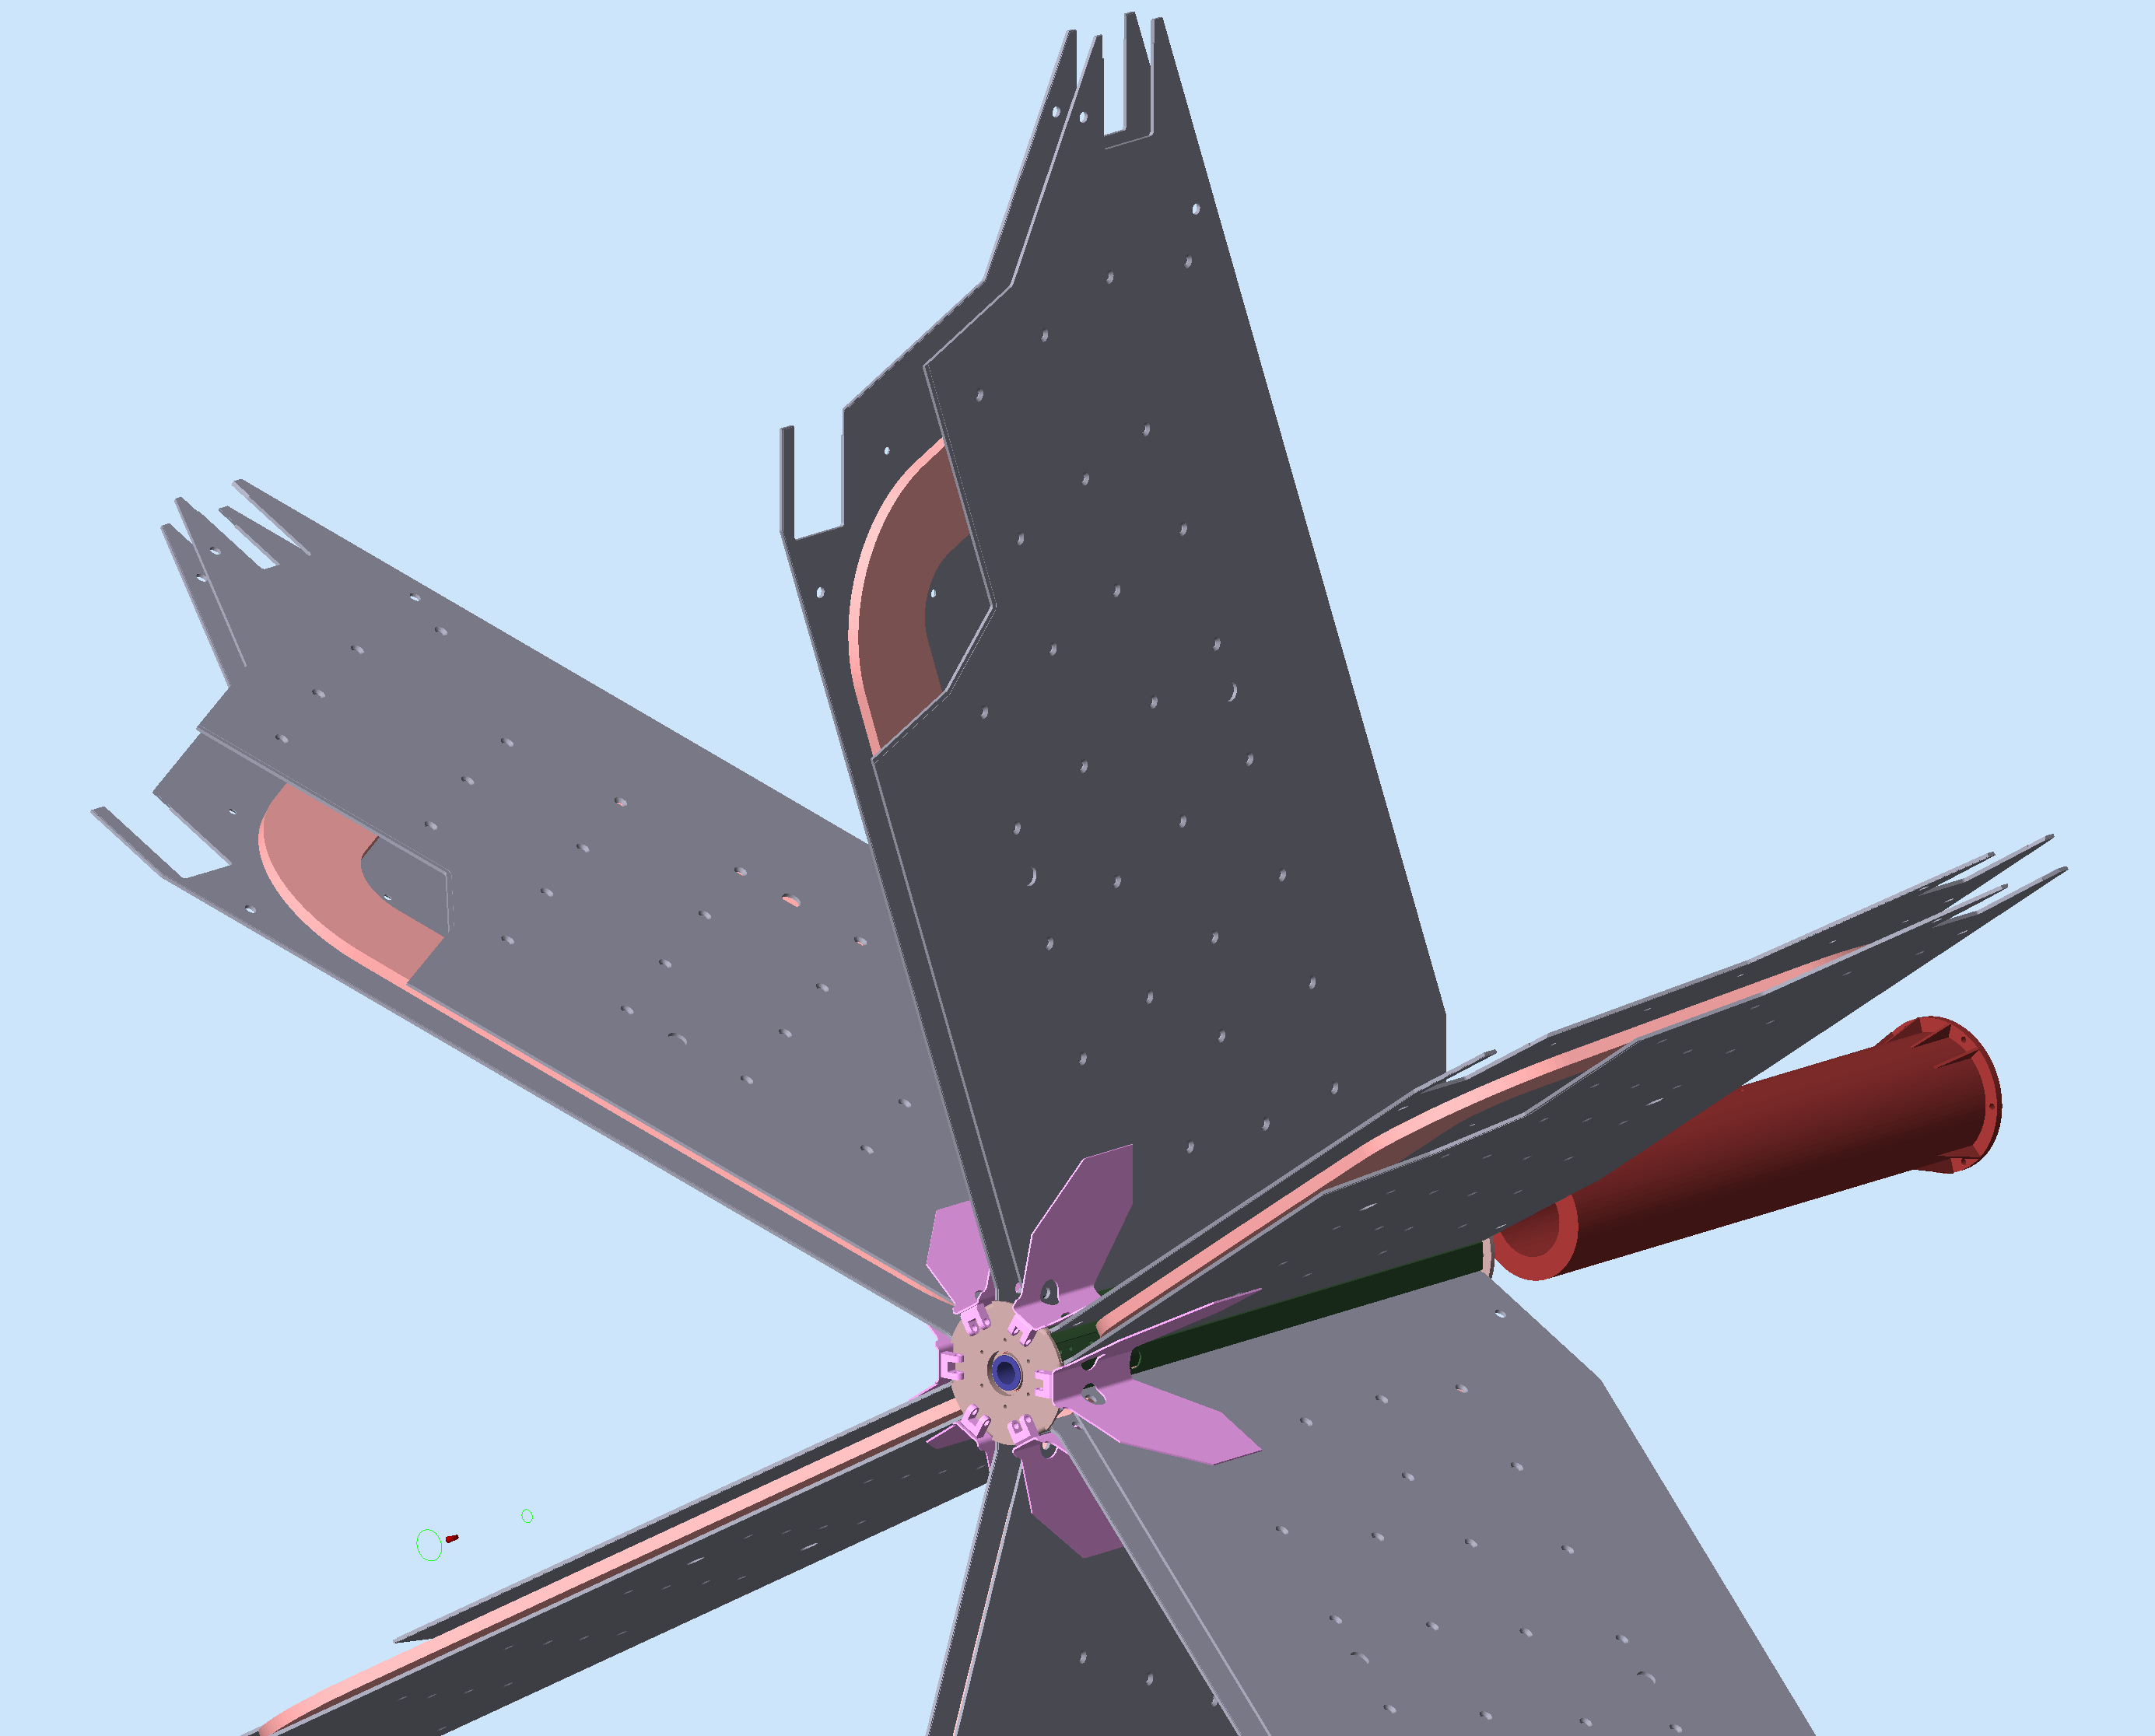
\includegraphics[width=0.95\columnwidth,keepaspectratio]{img/torusGeometry.png}
	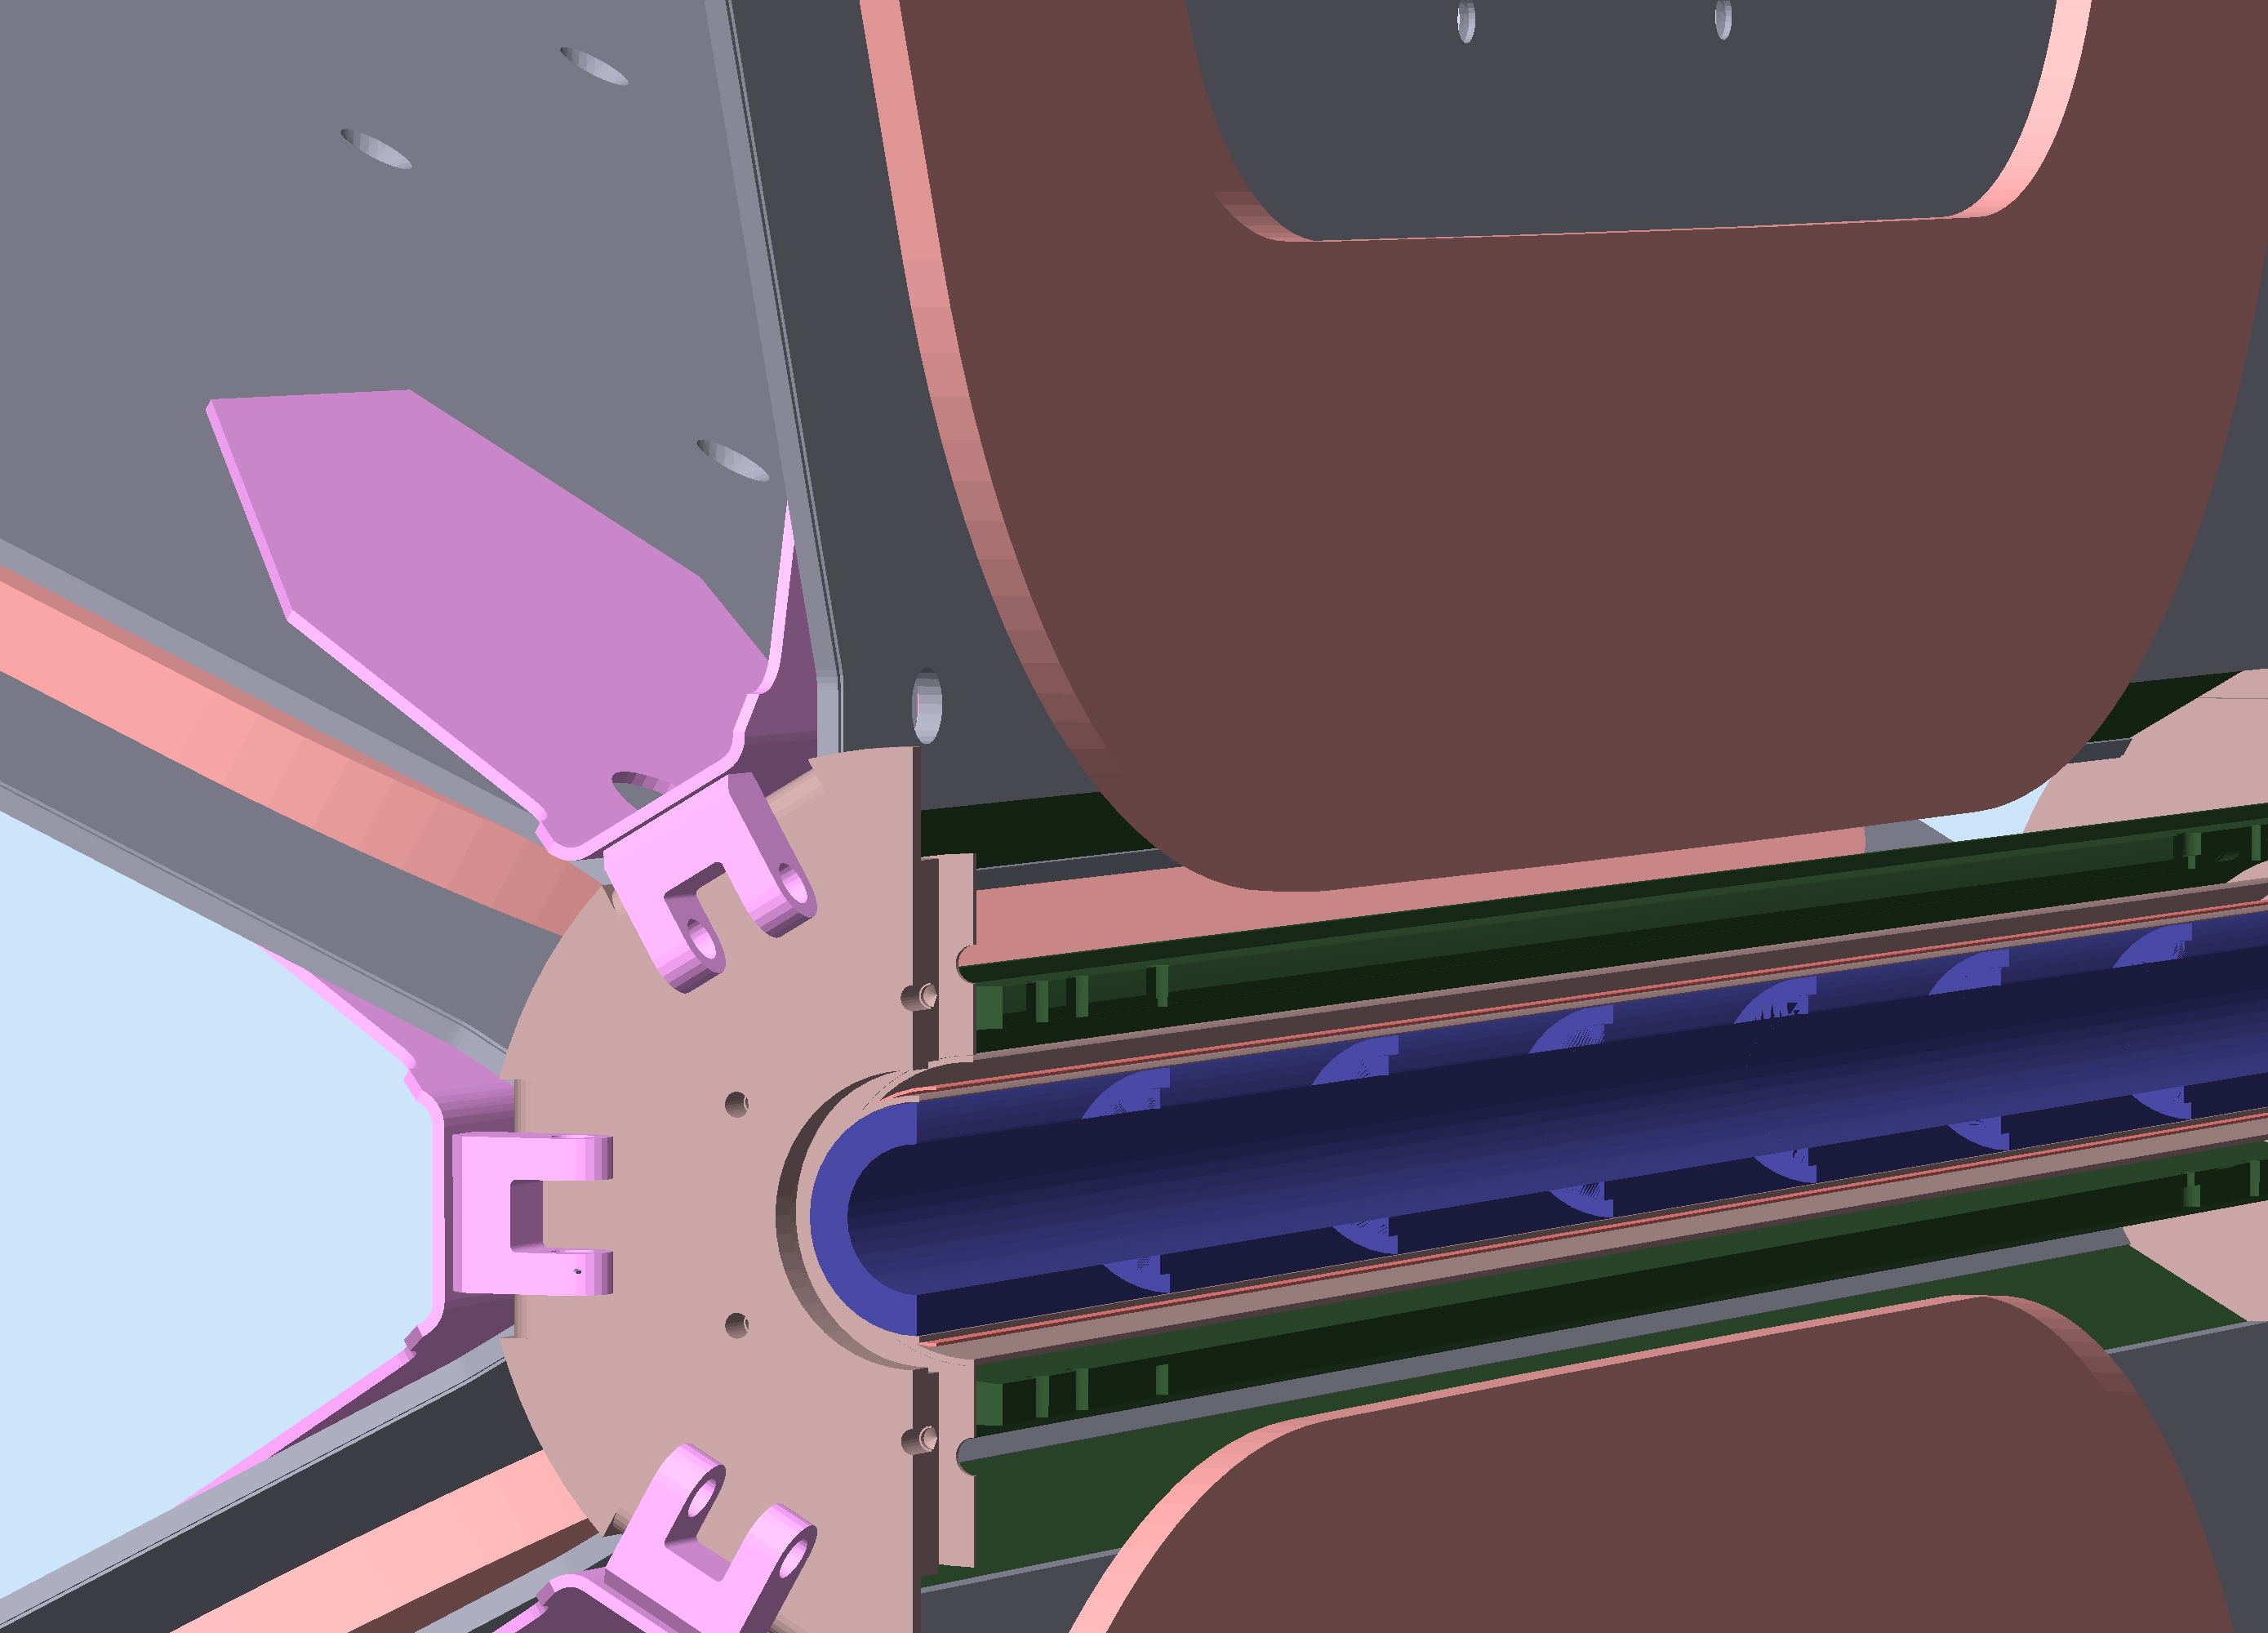
\includegraphics[width=0.95\columnwidth,keepaspectratio]{img/torusDetail.png}
	\caption{Top: the GEMC implementation of the torus hardware. The volumes are imported from the CAD engineering model.
            The stainless steel frame embeds the copper coils, immersed in the cold hub tube.
				Bottom: a section view of the torus in the vicinity of the beamline. The warm and cold hub are visible, along with the
				tungsten shielding (blue colors).}
	\label{fig:ecGeometry}
\end{figure}


\subsection{Magnetic Field Maps}



\subsubsection{Geometry Git Location}

